\section{Problem Definition}
\label{sec:problem}

In this section, we first give formal definitions related with knowledge base
and schema graph, then we define our praphrasing task in the optimization style,
at last, we prove that our problem is NP-Hard.

\begin{defn}[Knowledge Base]
A {\em knowledge base} is a tuple $\langle E, T, L, P, IsA \rangle$ where:
\begin{itemize}
  \item[*] $E$ is a finite set of all entities in $KB$.
  \item[*] $T$ is a finite set of all types in $KB$.
  \item[*] $L$ is a finite set of all predicate names in $KB$.
  All the entities, types and predicate names in $KB$ are identified by a unique id.
  \item[*] $P$ is a finite set of predicate instances with the form
  $p(e_1, e_2)$ where $e_1, e_2 \in E$ and $p \in L$.
  \item[*] $IsA$ indicates all types an entity belongs to, with the form $isa(e, t)$.
  Each entity has at least one type.
\end{itemize}
\end{defn}

%\KQ{Add some sentences showing what's a schema: abstraction}

%1. relation comes from a detail subgraph (give an example of mo_of)
A knowledge base is capable of representing complex relations between real entities.
\figref{fig:schemaExample}(a) shows an example instance of ``motherOf'' relation between
\textit{Barack Obama} and \textit{Ann Dunham}, which is actually a subgraph of $KB$.
Due to the semantic gap between knowledge base and natural language, there doesn't
exist a simple predicate describing mothers directly, however, $KB$ provides the
 ``female parent'' representation, which is the paraphrase of ``mother''.

%2. schema graph is a summarization o a list of subgraphs. (by substitution)
Intuitively, different instances of a complex relation shares a common structure,
which is an template of the complex relation. We call it as a \textit{schema graph}.

We define schema graph as follows.

%3. formal def. of S
\begin{defn}[Schema Graph]
A \textit{schema graph} $S$ is a tuple $\langle E', T', X, C, P_S \rangle$ where:
\begin{itemize}
  \item[*] $E' \subseteq E$, $T' \subseteq T$, which represent
  a subset of entities and types in KB respectively.
  \item[*] $X$ is a finite set of different variable entities, each $x \in X$
  indicates a placeholder for an entity $e \in E$. Each schema has
  two special variables, marked as $x_{subj}$ and $x_{obj}$,
  indicating the position of $e_1$ and $e_2$ coming from input entity pairs.
  \item[*] $C=\{\text{solid, dashed, isa}\}$, representing 3 different
  category labels of predicates in $S$.
  \item[*] $P_S$ is a finite set of \textit{schema predicates} with the
  form $p_s(v_1, v_2, c)$ where $v_1, v_2 \in E' \cup T' \cup X$, $c \in C$
  and $p_s \in L \cup \{\text{isa}\}$. Besides, the following constraints apply:
  \begin{itemize}
    \item[-] $c = \text{solid}$, if and only if $v_1, v_2 \in X$, $p_s \in L$,
    \item[-] $c = \text{dashed}$, if and only if $v_1 \in X, v_2 \in E'$, $p_s \in L$,
    \item[-] $c = \text{isa}$, if and only if $v_1 \in X, v_2 \in T'$ and $p_s = \text{isa}$.
  \end{itemize}
  %These restrictions make every predicate in $S$ connecting to at least one variable.
  %Generalize the definition. We do not need the graph to be a tree.

  %\item[*] All $solid$ predicates form a tree, where both $x_{subj}$ and $x_{obj}$ must
  %be a leaf, that is, linked by only one $solid$ predicate.
\end{itemize}
\end{defn}

%4. a small sentence describing the relation between S, G and hits.
A \textit{ground graph} is an instance of a schema graph $S$, with
every variable $x_i$ substituted by a concrete entity $e_i$,
such that the resulting graph is a subgraph of $KB$.
\figref{fig:schemaExample}(b) shows the schema graph of ``motherOf'' relation,
\figref{fig:schemaExample}(a) is one of its ground graphs.
% \KZ{Consider swapping the position of (a) and (b) in the figure.}

\begin{figure}[h]
\centering
\epsfig{file=schemaExample.eps, width=0.95\columnwidth}
\caption{Example ground graph and schema graph for ``motherOf'' relation}
\label{fig:schemaExample}
\end{figure}

Obviously, each ground graph indicates a complex relation between entity pair 
$\langle e_{subj}, e_{obj} \rangle$ (the specific entities at $x_{subj}$ and $x_{obj}$ position).
Grouping all ground graphs, we define the \textit{hit pairs} of a schema:

%5. formal def. of Hits. (S, G1, G2, ... ==> HP(S))
\begin{defn}[Hit Pairs]
Let $S$ be a schema and $G$ be a ground graph of $S$. The entity pair $\langle e_{subj}, e_{obj} \rangle$
is a $hit$ of $S$. In addition, $HP(S)$ is the \textit{hit pairs} of $S$, which is a set of all hits derived from
each ground graph of $S$.
\end{defn}


%\KQ{Put example $S$ here, one for running example, another one for the most simple
%schema covering $|E|^2$ entity pairs.}
%
%A ground graph $G$ is generated from its underlying schema graph $S$, where
%each variable $x$ is instantiated with an entity $e_x \in E$, such that:
%\begin{itemize}
%  \item[-] $\forall p_s(x_1, x_2, \text{solid}) \in P_S,~ p_s(e_{x_1}, e_{x_2}) \in P$,
%  \item[-] $\forall p_s(x, e, \text{dashed}) \in P_S,~ p_s(e_x, e) \in P$,
%  \item[-] $\forall p_s(x, t, \text{ida\_dashed}) \in P_S,~ t \in IsA(e_x)$.
%\end{itemize}
%\noindent
%Actually $G$ is a subgraph of $KB$ with the position of subject and object specified.
%We call the entity pair $\langle e_{subj}, e_{obj} \rangle$ a hit of $G$ and its underlying $S$.
%Grouping each $G$ derived from $S$, we define $HP(S)$ as the set of all hits of $S$.

%1. task is ...
Our task of paraphrasing between NL and KB is to find a set of \textit{output schemas} for
describing a given list of entity pairs.
Output schemas are chosen from a set of \textit{candidate schemas} in KB,
which are the most suitable (neither too general nor too specific) for the given data.

In order to describe all given entity pairs, the hit pairs of output schemas
must cover all the given entities.
Furthermore, we build a cost function to measure the fitness score over a schema and entity pairs,
turning our task to an optimization problem.
%2. bridge the gap bet. entity and schema. that's assign
%A ground graph bridges the gap between $\langle e_{subj}, e_{obj} \rangle$ and a schema.
%All schemas that can hit at least one entity pair form the schema searching space.
%Each entity pair is assigned to at least one schema which hits the pair.
%After the step of assignment, a cost is produced when a schema is selected
%to describe all its assigned entity pairs assigned.
%%3. Goal: Min Cost
%With cost function provided, we look for a set of schemas describing
%all entity pairs at a minimum cost.

%4. Formally Define.
The following is the formal definition of our task.

\begin{defn}[The Paraphrasing Problem]
\label{def:pp}
Given $KB$, entity pairs $EP = \{ep_1, ..., ep_n\}$,
a cost function $f: EP \times S \rightarrow [0, +\infty)$,
and a function $sel$ that selects all candidate schemas ($CS$) from $KB$,
return a set of output schemas $OS \subseteq CS$, such that:
\begin{itemize}
    \item[-] $EP \subseteq \bigcup_{S \in OS} HP(S)$,
    \item[-] Whole cost $Z = \sum\nolimits_{S \in OS} f(EP, S)$ is minimum.
\end{itemize}
%
%Given $KB$, a binary relation pattern $rel$ with its support entity pairs
%$EP = \{ ep_1, ..., ep_n \}$, cost function $f$ and $g$,
%Let $CS = \{S | EP \cap HP(S) \neq \emptyset \}$ be \textit{candidate schemas} and
%$DS = \{S_1, ..., S_m\} \subseteq CS$ be a set of \textit{selected schemas}.
%Let $Ass_{m \times n}$ be an 0/1 \textit{assignment matrix} from $EP$ to $DS$ and
%\textit{support set} $sup(S_j) = \{ep_i | Ass_{ij} = 1\}$ be all entity pairs assigned to the $j$-th schema.
%The assignment $Ass$ is a valid assignment over $EP$ and $SG$ if it satisfies the following
%constraints:
%\begin{itemize}
%    \item[-] $Ass_{ij} = 1 \Rightarrow ep_i \in HP(S_j)$,
%    \item[-] $\forall ep_i \in EP, \exists S_j \in DS, Ass_{ij} = 1$,
%    \item[-] $\forall S_j \in DS, \exists ep_i \in EP, Ass_{ij} = 1$,
%\end{itemize}
\end{defn}

%The selected schemas $DS$ and corresponding $Ass$ are optimal, if it minimizes
%the cost $Z(DS, Ass) = \sum\nolimits_{S \in DS} f(S) + g(S, sup(S))$ , where $f$ is a
%cost function over a specific schema, and $g$ is a cost function over a schema along
%with its support set. Both $f$ and $g$ are non-negative functions and defined by users.

%Now we define the task of paraphrasing between NL and KB. Given KB, a binary relation
%pattern $rel$ with its support entity pairs
%$EP = \{\langle e_1^{(1)}, e_2^{(1)} \rangle , ..., \langle e_1^{(n)}, e_2^{(n)} \rangle \}$
%from KB, we want to find a set of schema graphs $\vec{S}$ that:
%
%\begin{itemize}
%    \item[-] Each entity pair is hit by at least one schema in $\vec{S}$,
%    \item[-] The schemas fits $EP$ at the best (neither too general nor too specific).
%\end{itemize}
%
%where the score of fitness is produced by a cost function $Cost(EP, \vec{S})$.
%The cost function captures both compactness and precision for the set of schemas to describe the entity pairs.


%\KQ{The reason of restricting at most K schema graphs is to avoid generating too many schemas.
%In the formula, Cost(EP|S) is the dominant one,
%probably 5~10 pairs hit by one specific schema could bring that schema into description set.}

Next, we prove that the paraphrasing problem is NP-Hard.
We show that by constraining $sel$ and $f$ to some specific classes of
functions, the resulting instance of the paraphrasing problem can
be reduced from the well-known {\em weighted set cover problem},
which is NP-complete.

\begin{thm}
Given $KB$, $EP$, candidate selecting function $sel$ and cost function $f$,
computing the optimal output schemas for describing all pairs in $EP$, is NP-Hard.
\end{thm}

\begin{proof}
%Rephrase that a simplified instance of our problem is still NP-Hard.
We first state the simplified instance of the paraphrasing problem.
The function $sel$ is restricted by only returning a special kind
of schema, which has only $x_{subj}$ and $x_{obj}$ connected by a solid
predicate. In addition, the cost function $f$ is simplified as
$g: S \rightarrow [0, \infty)$, that is,
the cost is only determined by the schema, and not by EP.

After the simplification, the \textbf{decision version} of the
paraphrasing problem is as follows:
Given $KB$, $EP$, $sel$, $g$ and a threshold $\theta$, is there a set of output schema $OS$
covering all pairs in $EP$, such that whole cost $Z \leq \theta$ ?
The proof relies on a reduction from \textsc{Weighted Set Cover} problem:
Given a universe $U = \{u_1, ..., u_n\}$, a threshold $\theta$, a set $V = \{v_1, ..., v_m\}$
whose union equals to $U$, each $v_j \subseteq U$ and a weight set $W = \{w_1, ..., w_m\}$ assigned to each $v_j$,
is there a cover $C \subseteq V$ whose union equals to $U$, and the summation weight is no larger than $\theta$ ?

\textit{Reduction:} For an arbitrary instance of \textsc{Weighted Set Cover} problem,
we build a $KB$ based on $U$ and $V$, where it contains only $m$ different predicates $p_1, ..., p_m$,
leading to a set $m$ simple candidate schemas.
We map each $u_i$ to an entity pair $ep_i = \langle e_{subj}^{(i)}, e_{obj}^{(i)} \rangle $.
For any $u_i$ and $v_j$, if $u_i \in v_j$, we add a predicate instance $p_i(e_{subj}^{(i)}, e_{obj}^{(i)})$ into $KB$.
Finally, we define the cost function as $g(S_j) = w_j$ for each schema.

Since all schemas have only one edge, retrieving candidate schemas from $KB$
along with hit pairs can be done in polynomial time. Therefore, the paraphrasing decision problem
is formulated as: Given $n$ entity pairs and $m$ sets of hit pairs whose union cover all pairs,
with the weight $w_j$ assigned to the $j$-th set, can I pick some sets that still cover all
the entity pairs, satisfying the summation weight no larger than $\theta$ ?
Obviously, solving this paraphrasing decision problem is equivalent to
solving the corresponding \textsc{Weighted Set Cover} problem.
\end{proof}

%In this reduction, $U$ and $V$ are used to construct a $KB$,
%where $m$ different predicates $p_1, ..., p_m$ are in $KB$,
%each $u_i$ indicates an entity pair $\langle e_1^{(i)}, e_2^{(i)} \rangle $,
%and the relation instance $p_i(e_1^{(i)}, e_2^{(i)})$ is contained (or not) in $KB$
%according to whether $u_i$ is covered by $S_j$.
%Since we only consider the schema with one solid edge,
%the complexity of finding all \textit{candidate schemas} of these $n$ entity pairs
%is within polynomial time, where the $j$-th candidate schema hits those corresponding entity pairs within $V_j$,
%with the cost function $f(S_j) = w_j$.
%In addition, since the function $g$ is always zero, the assignment step could be ignored (if $S_j$ is selected,
%then all its hitting pairs would be assigned it without bringing extra costs).
%Therefore, if there exists a cover $C$ satisfying the $\theta$ limit, then
%it's possible to select schemas covering all entity pairs with cost no more than $\theta$.
